\documentclass[]{article}
\usepackage{lmodern}
\usepackage{amssymb,amsmath}
\usepackage{ifxetex,ifluatex}
\usepackage{fixltx2e} % provides \textsubscript
\ifnum 0\ifxetex 1\fi\ifluatex 1\fi=0 % if pdftex
  \usepackage[T1]{fontenc}
  \usepackage[utf8]{inputenc}
\else % if luatex or xelatex
  \ifxetex
    \usepackage{mathspec}
  \else
    \usepackage{fontspec}
  \fi
  \defaultfontfeatures{Ligatures=TeX,Scale=MatchLowercase}
\fi
% use upquote if available, for straight quotes in verbatim environments
\IfFileExists{upquote.sty}{\usepackage{upquote}}{}
% use microtype if available
\IfFileExists{microtype.sty}{%
\usepackage{microtype}
\UseMicrotypeSet[protrusion]{basicmath} % disable protrusion for tt fonts
}{}
\usepackage[margin=1in]{geometry}
\usepackage{hyperref}
\PassOptionsToPackage{usenames,dvipsnames}{color} % color is loaded by hyperref
\hypersetup{unicode=true,
            pdftitle={CWRU DSCI351-451: Exploratory Data Science},
            pdfauthor={Prof.:Roger French, TA:JiQi Liu},
            colorlinks=true,
            linkcolor=Maroon,
            citecolor=Blue,
            urlcolor=blue,
            breaklinks=true}
\urlstyle{same}  % don't use monospace font for urls
\usepackage{graphicx,grffile}
\makeatletter
\def\maxwidth{\ifdim\Gin@nat@width>\linewidth\linewidth\else\Gin@nat@width\fi}
\def\maxheight{\ifdim\Gin@nat@height>\textheight\textheight\else\Gin@nat@height\fi}
\makeatother
% Scale images if necessary, so that they will not overflow the page
% margins by default, and it is still possible to overwrite the defaults
% using explicit options in \includegraphics[width, height, ...]{}
\setkeys{Gin}{width=\maxwidth,height=\maxheight,keepaspectratio}
\IfFileExists{parskip.sty}{%
\usepackage{parskip}
}{% else
\setlength{\parindent}{0pt}
\setlength{\parskip}{6pt plus 2pt minus 1pt}
}
\setlength{\emergencystretch}{3em}  % prevent overfull lines
\providecommand{\tightlist}{%
  \setlength{\itemsep}{0pt}\setlength{\parskip}{0pt}}
\setcounter{secnumdepth}{5}
% Redefines (sub)paragraphs to behave more like sections
\ifx\paragraph\undefined\else
\let\oldparagraph\paragraph
\renewcommand{\paragraph}[1]{\oldparagraph{#1}\mbox{}}
\fi
\ifx\subparagraph\undefined\else
\let\oldsubparagraph\subparagraph
\renewcommand{\subparagraph}[1]{\oldsubparagraph{#1}\mbox{}}
\fi

%%% Use protect on footnotes to avoid problems with footnotes in titles
\let\rmarkdownfootnote\footnote%
\def\footnote{\protect\rmarkdownfootnote}

%%% Change title format to be more compact
\usepackage{titling}

% Create subtitle command for use in maketitle
\newcommand{\subtitle}[1]{
  \posttitle{
    \begin{center}\large#1\end{center}
    }
}

\setlength{\droptitle}{-2em}

  \title{CWRU DSCI351-451: Exploratory Data Science}
    \pretitle{\vspace{\droptitle}\centering\huge}
  \posttitle{\par}
    \author{Prof.:Roger French, TA:JiQi Liu}
    \preauthor{\centering\large\emph}
  \postauthor{\par}
      \predate{\centering\large\emph}
  \postdate{\par}
    \date{04 September, 2018}


\begin{document}
\maketitle

{
\hypersetup{linkcolor=black}
\setcounter{tocdepth}{6}
\tableofcontents
}
\setcounter{section}{2} \setcounter{subsection}{1}
\setcounter{subsubsection}{1}

\hypertarget{reading-homeworks-projects-semprojects}{%
\paragraph{Reading, Homeworks, Projects,
SemProjects}\label{reading-homeworks-projects-semprojects}}

\begin{itemize}
\item
  Readings:

  \begin{itemize}
  \tightlist
  \item
    for today: RPR 35-64
  \item
    For Thursday RPR 65-93
  \end{itemize}
\item
  Homeworks

  \begin{itemize}
  \tightlist
  \item
    HW1 due today
  \item
    HW2 available on Thursday
  \end{itemize}
\item
  Data Science Projects:
\item
  451 SemProjects:
\item
  Friday Comm. Hour
\end{itemize}

\hypertarget{textbooks}{%
\paragraph{Textbooks}\label{textbooks}}

\begin{itemize}
\tightlist
\item
  \href{https://play.google.com/books/reader?printsec=frontcover\&output=reader\&id=F1mVHgAAAEAJ\&pg=GBS.PA1}{Peng:
  R Programming for Data Science}
\item
  \href{https://play.google.com/books/reader?printsec=frontcover\&output=reader\&id=R-09BgAAAEAJ\&pg=GBS.PA1}{Peng:
  Exploratory Data Analysis with R}
\item
  \href{https://play.google.com/books/reader?printsec=frontcover\&output=reader\&id=G2EOBwAAAEAJ\&pg=GBS.PA0}{Open
  Intro Stats, v3}
\item
  \href{https://play.google.com/books/reader?printsec=frontcover\&output=reader\&id=I6y3DQAAQBAJ\&pg=GBS.PA1}{Wickham:
  R for Data Science}
\item
  \href{https://play.google.com/books/reader?printsec=frontcover\&output=reader\&id=KtuPCwAAAEAJ\&pg=GBS.PA0}{Hastie:
  Intro to Statistical Learning with R}
\end{itemize}

\hypertarget{syllabus}{%
\paragraph{Syllabus}\label{syllabus}}

\begin{figure}
\centering
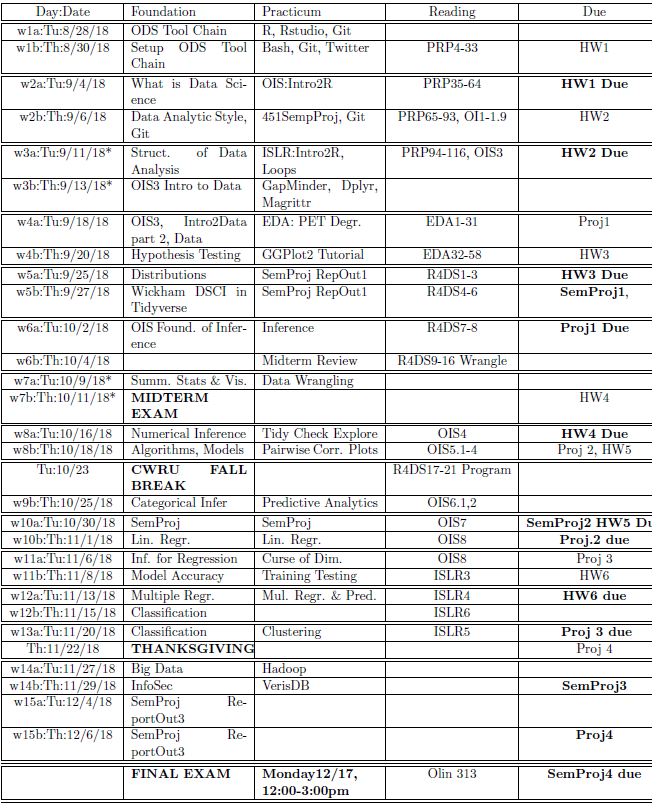
\includegraphics{./figs/syllabus.png}
\caption{DSCI353-453 Syllabus}
\end{figure}

\hypertarget{links}{%
\subsubsection{Links}\label{links}}


\end{document}
